\documentclass[letterpaper, 12pt]{article}

\usepackage[in]{fullpage}
\usepackage{multicol}
\usepackage{mdwlist}
\usepackage{hyperref}
\usepackage{graphicx}
\usepackage{tabularx}
\usepackage{multirow}

\pagestyle{empty}

\begin{document}

\begin{flushleft}
Path-finding with Dijkstra's Algorithm\\
Benjamin Woodruff\\
\href{mailto:odetopi.e@gmail.com}{odetopi.e@gmail.com},
Duncan U.~Fletcher High School
\end{flushleft}

\vspace{0.25in}

\begin{huge}
    \begin{center}
        \textbf{Path-finding with Dijkstra's Algorithm}
    \end{center}
\end{huge}
\vspace{.5in}

\begin{multicols}{2}

\section{Abstract}

As we develop and advance in the Botball competition, the need arises to build
more and more intelligent systems. Path-finding isn't only about reducing the
repetitive work on programmers, but also allowing robots to make decisions on
the fly. As an alternative to techniques such as line-following, or as an aid,
path-finding can take advantage of the largely static Botball board layout. This
paper seeks to describe a technique and example implementation by which a
perfectly optimal, non-intersecting, easily navigable path can be found. In
addition, this document outlines surrounding support systems for working with
such paths, and putting things into practice.

\section{Reasoning}

\subsection{An Example Problem}

Imagine you have a movement library, such as CBCJVM's, that allows for simple
geometric movements, as well as position tracking. The robot successfully finds
a set of blocks with it's camera, but now you have to figure out how to navigate
back to your drop-off point. There's a few simple answers, such as reversing the
movements that you took to get the blocks, returning you to a known point, but
all of these are inefficient. If you try to simply move from one point to
another, using position tracking, you have no easy way of handling if there is
an object in the way of your path.

\subsection{How Pathfinding can Help}

A proper path-finding system already knows the layout of obstacles on the board,
either through static (programmer) input, or through dynamically (sensor)
inputted information. With this, the system should be able to determine the best
way to get from Point A to Point B, avoiding everything else in-between. This
can then be distilled into a simple set of actions, such as

\begin{enumerate*}
    \item Rotate 37 degrees clockwise
    \item Move 36 cm forward
    \item Rotate 84 degrees counter-clockwise
    \item Move 15 cm forward
\end{enumerate*}

\section{A* (A-Star)}

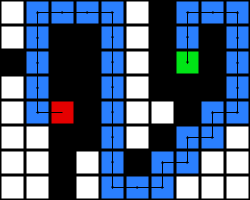
\includegraphics[width=\columnwidth]{img/a_star.pdf}

The typical way of solving such a problem, as has been done by teams such as
Norman High School in the past, has been to turn the board into a grid, and to
utilize the simple A* algorithm to then generate a path on the grid. Such a path
is then traced and turned into a set of movements, like above.

However, such a system works in a non-optimal manner. Our robots do not operate
on a grid, and, as a result, the generated paths can end up including far more
points than ideal. Additionally, the A* algorithm does not guarantee that the
resultant path, even in a grid setting, is the shortest one.

While this is an interesting system to work with, and an even more interesting
proof of concept, the more geometrically aligned Dijkstra's algorithm appears a
better choice.

\section{Graph Theory}

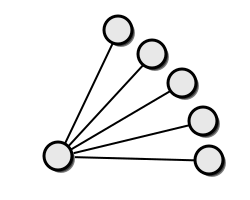
\includegraphics[width=\columnwidth]{img/graph_theory.pdf}

Let's start by turning the board into the simplest representation we can: a set
of line segments. Each of these line segments have two end-points, or nodes, and
a group of lines, sharing nodes at vertices form polygons. The board can be
represented through a set of inaccessible polygon areas, and otherwise open
area.

When you are forming an optimal path, assuming the robot itself is a point-mass,
the only nodes included in the path will be the starting point, the ending
point, and the vertices of the polygons on the map. This assumption greatly
reduces our search-space.

\subsection{Line-of-Sight}

As obvious as it seems to us that the robot cannot simply pass through pvc-pipe
(excluding robots with treads or other advance apparatuses), we must define such
in our algorithm. The obvious way of doing such is to declare that from one
node, the only other directly accessible nodes are those within the line-of-
sight of the current node.

Looking around, there don't seem to be many good published line-of-sight
algorithms for our purposes. Most, often for graphical setups, deal with pixel-
level, or grid-based systems.

As a result, I attempted, with quite some success, a naive technique, derived
from ray-tracing systems.

\subsubsection{Ray-Tracing}

Ray-tracing is a common technique for high quality 3d rendering, and such
algorithms lay at the center of multi-million dollar programs, such as Pixar's
Renderman software, used in countless Disney-Pixar flicks, as well as a wide
variety of other Hollywood blockbusters.

The algorithm is a near brute-force approach at mimicking mother-nature. We can
pretend that the sun, instead of sending out continuous particle-waves, sends
out countless numbers of rays, which follow rules of refraction. Some of these
end up in our view, others don't. The density of returned ``rays'' per unit area
(per pixel) determines the resultant brightness. If rays don't get to a certain
area, we end up with shadows (See where we're going?).

\subsubsection{Reverse Ray-Tracing}

One might say this implementation is extremely inefficient, and it is. Many of
the rays get lost in the abyss of the computer's RAM. Perhaps they enter the
world of Tron, and get taken into the games, to be tortured, only to be killed
by the evil garbage collector (After all, we're using a high-level managed
language like Java, right? If not, imagine it's the dark lord
\texttt{dealloc}.).

As a result, there's an alternative strategy, although not always applicable, or
as ideal. If, for example, the light-source is located at the same point as the
view-point, we can have each of our objects send emit rays back towards the
view-point, instead of the other way around, hence the algorithm's name. Along
the way, they can collide with other objects and such, but not near as many rays
are wasted, and such an algorithm is now far from brute-force. Such an algorithm
is typically \(\mathrm{O}(n)\), where \(n\) is the number of objects in the
field.

\subsubsection{Lighting up the Board}

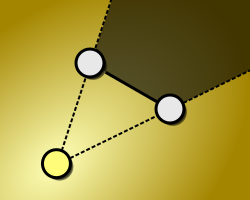
\includegraphics[width=\columnwidth]{img/light.pdf}

Imagine the robot is acting as a lamp on the board. If it sends off rays of
light, only the ones intersecting with walls, or lines, are stopped, and all
other rays continue traveling infinitely.

\subsubsection{Reverse Ray-Tracing and Line of Sight}

Let's have each node on the board draw a line segment to the current node on the
board. From there, we can check to see if this line segment drawn intersects any
polygons on the board. If it does, then we can conclude that the node is not
directly visible or accessible.

\subsection{Dijkstra's Algorithm}

nom

\end{multicols}

\begin{tabularx}{\textwidth}{l|X|XXXX|}
	\cline{2-6}
	\multirow{2}{*}{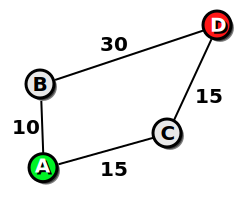
\includegraphics{img/dijksra.pdf}} &
	 \multirow{2}{*}{\textbf{From}}&\multicolumn{3}{c|}{\textbf{To}}\\\cline{3-6}
	&                              & A & B & C & D \\ \cline{2-6}
\end{tabularx}

\end{document}
